\documentclass[11pt]{article}

\usepackage{preamble}


\begin{document}
    \begin{titlepage}
        \center
        % University
        \textsc{\LARGE University of Moratuwa}\\[.5cm]

        % Document info
        \textsc{\Large Circuits And System Design}\\[0.2cm]
        \textsc{\large EN3030}\\[1cm]                                        % Course Code
        \HRule \\[0.4cm]
        { \Large \bfseries ASSIGNMENT : WEEK 01}\\[0.25cm]
        \HRule \\[1cm]
        \large
        \textbf{\emph{\large Team : INFOS}}\\
        [0.3cm]
        \begin{tabular}{ |l| c|c| }
            \toprule
            Yasarathna D.D.K.B. & 190719V & Ex - 01 \\
            \midrule
            Tharindu.O.K.D      & 190622R & Ex - 02 \\
            \midrule
            S.Sanjith           & 190562G & Ex - 03 \\
            \midrule
            K.Kajhanan          & 190286M & Ex - 04 \\
            \midrule
        \end{tabular}\\
        [.5cm]
        {\large \today}\\[1cm]
        
\includegraphics[width=0.4\textwidth]{mora.png}\\[1cm]    % University logo
        \tableofcontents
        \vfill
        \HRule
        \flushleft {Executable codes can be found \href{https://gist.github.com/sanjith1999/62c41b6aa1321804bc55865d851566a7}{here}}
    \end{titlepage}


    \section{Ripple Carry Adder \& Pipelined Architecture}
    The following discussion will illustrate the improvement in the performance of the adder in adding four
    32-bit numbers consecutively. Adders are formed using four separate eight-bit adders and results are based
    on giving inputs in two different passions in a way to evaluate the effect of pipelining over performance.
    For the comparison purposes the average gate delay is considered as $\tau$.

    \subsection{Operation in Normal Mode}
    A full adder takes at least 2$\tau$ from the time its inputs are available, to ensure useful results are
    in place. This way propagation of carry-value throughout the blocks leads to a delay of 16$\tau$ for an
    8-bit adder. Hence an addition between two 32-bit numbers takes $4\times 16\tau = 64\tau$.

    \begin{figure}[h]
        \begin{center}
            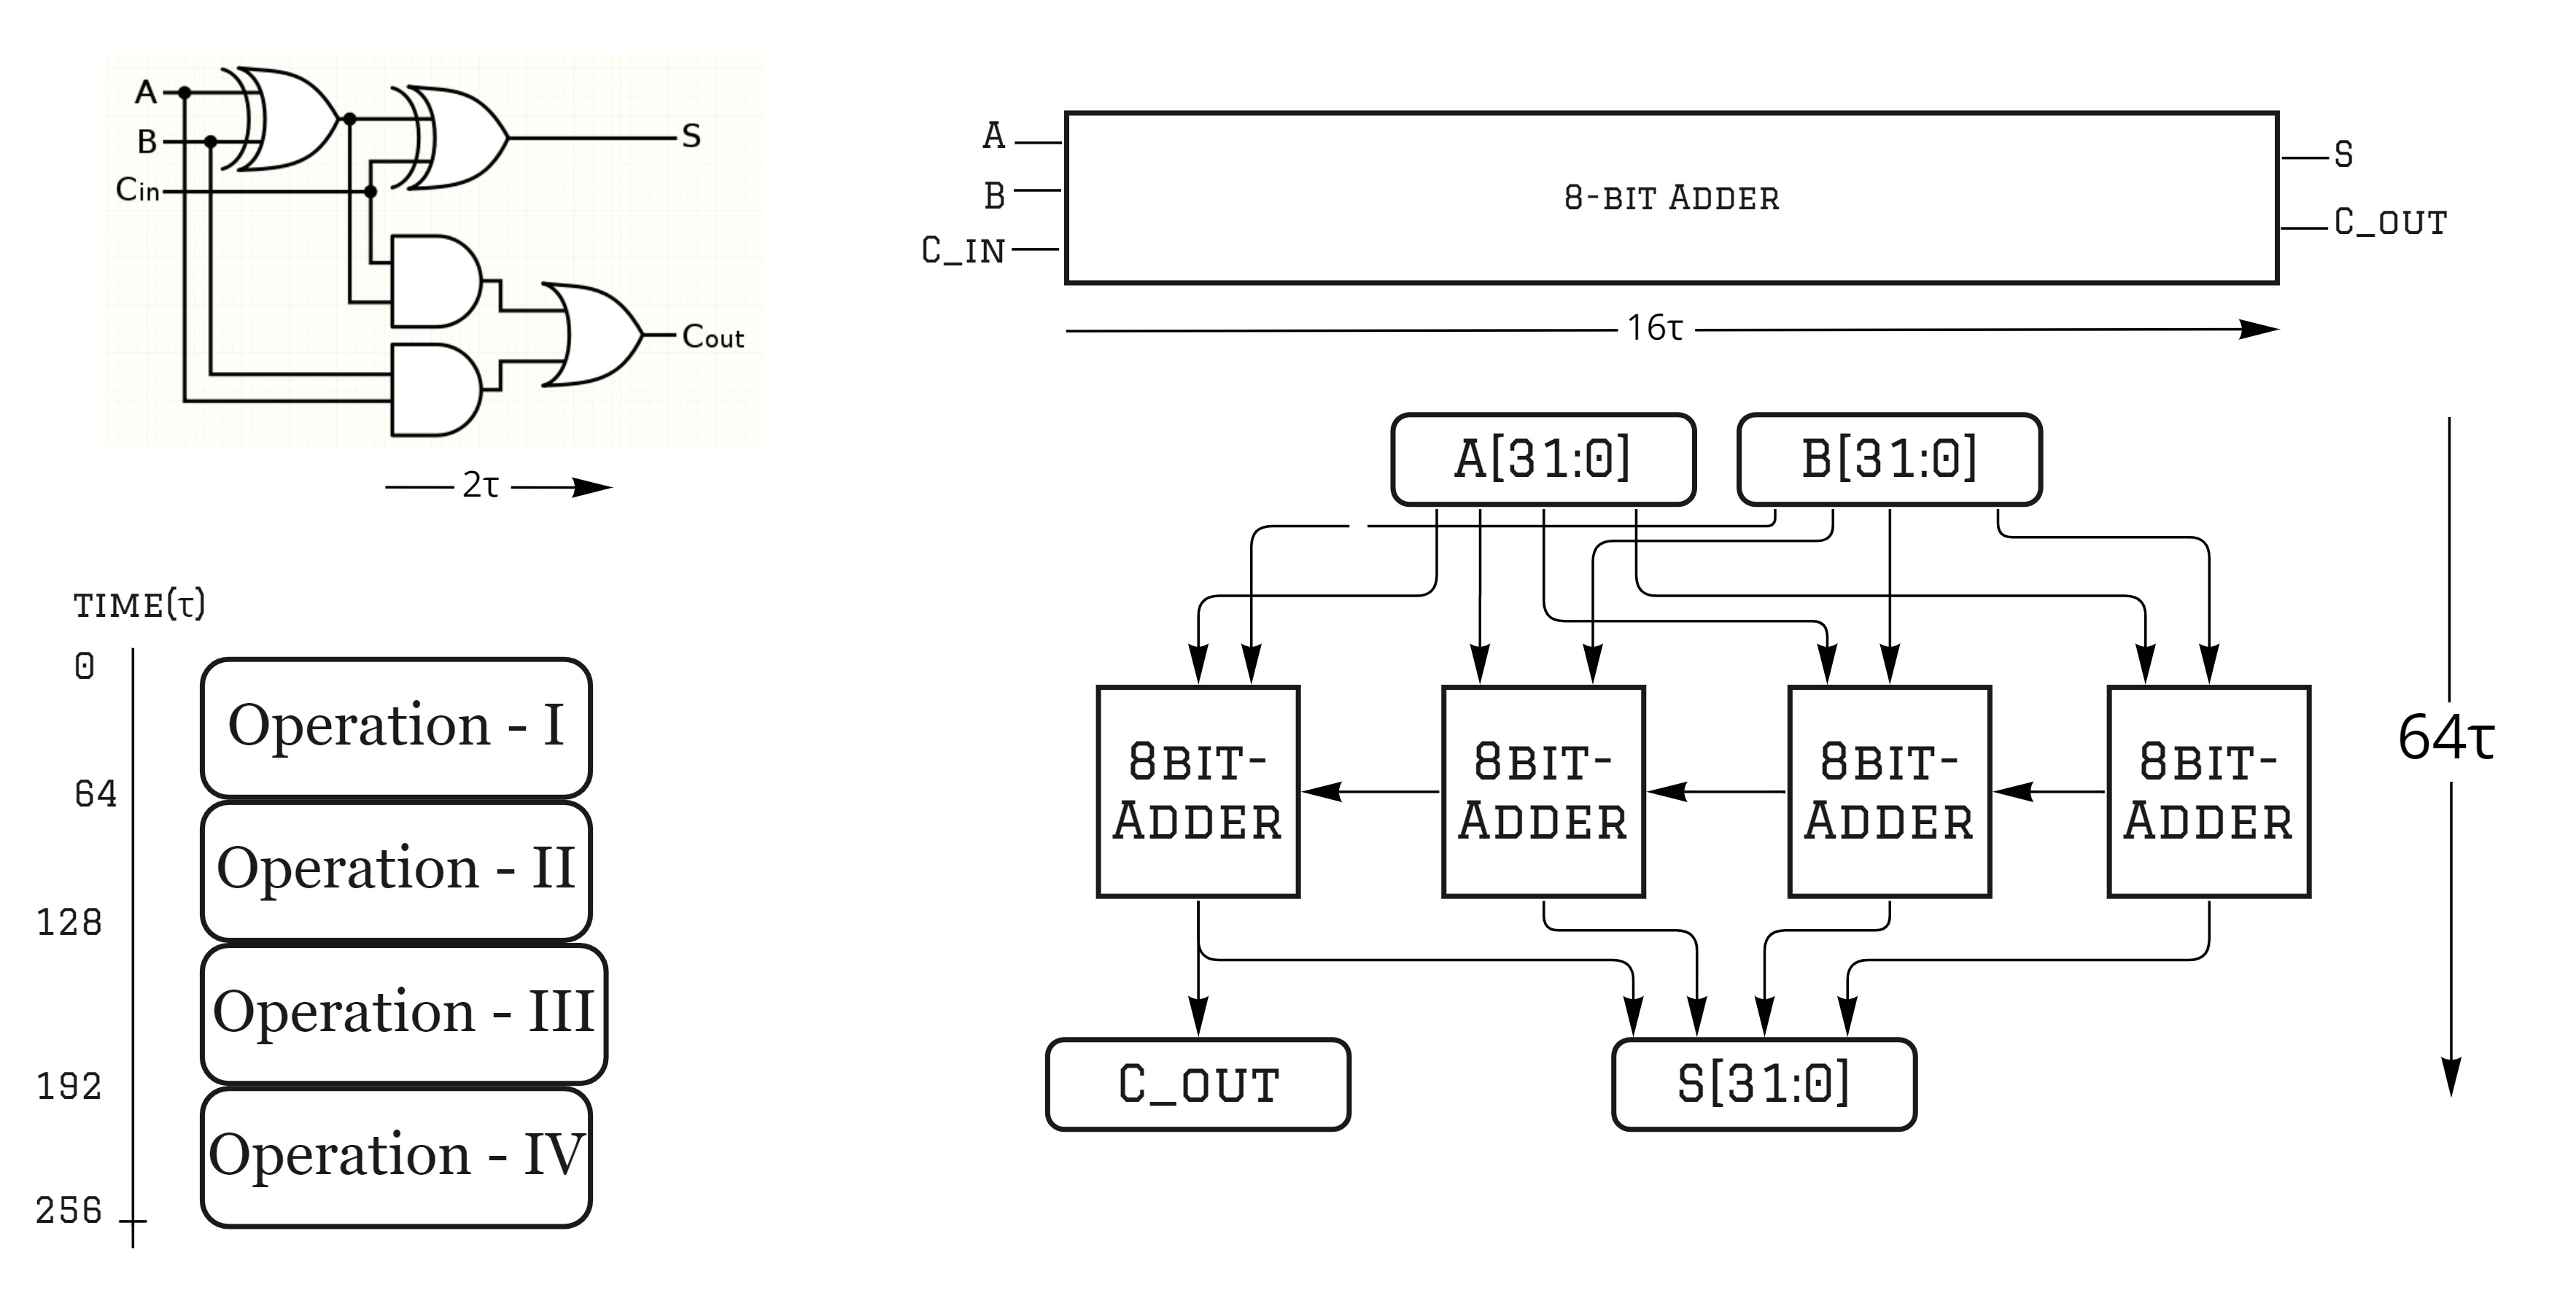
\includegraphics[width=.85\textwidth]{ripple_adder}
            \caption*{$\text{Total time taken by adder to perform four consecutive addition} = 4\times 64\tau = 256\tau$}
        \end{center}
    \end{figure}
    \vspace{-.5cm}

    \subsection{Pipelined Architecture}
    \vspace{-.5cm}
    \begin{figure}[h]
        \begin{minipage}{.7\textwidth}
            \begin{center}
                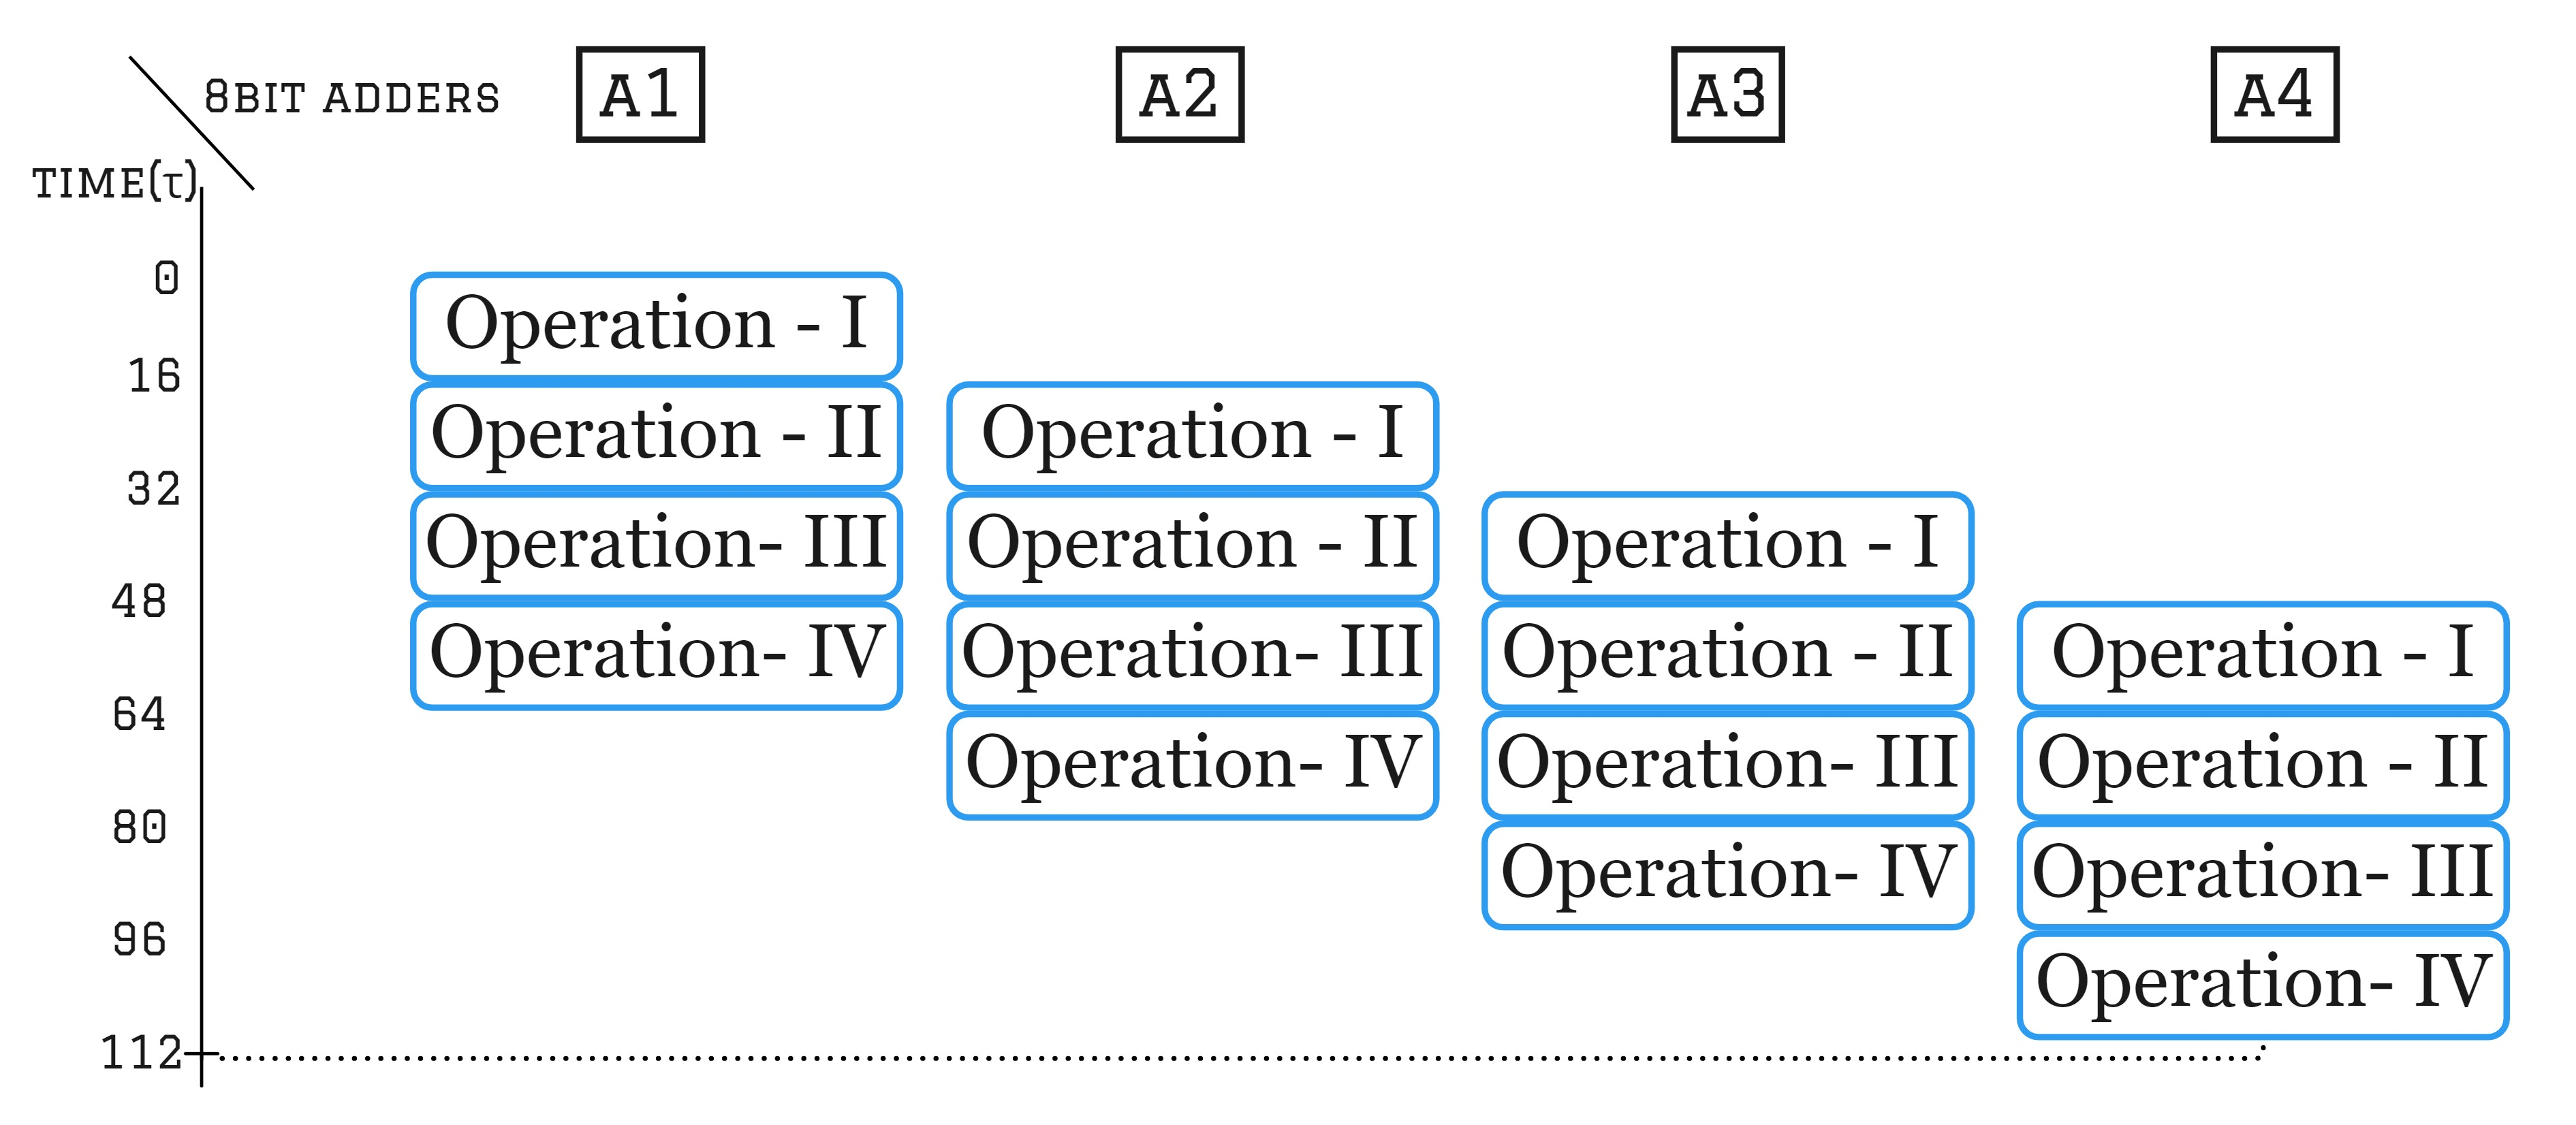
\includegraphics[width=.95\columnwidth]{pipe_des}
                \caption*{Total Time taken = 112$\tau$}
            \end{center}
        \end{minipage}
        \begin{minipage}{.28\textwidth}
            The Main idea of pipelining is rather than waiting for the whole operation about one addition to complete, make use of
            the unutilized 8-bit adder blocks to perform the subsequent calculations.In the case of four
            additions, utilizing idle stages in the adder blocks seem to reduce the accumulated
            gate delays from 256$\tau$ low to 112$\tau$.
        \end{minipage}
        \newline
        \caption*{Simulation Results}
        \begin{minipage}{.48\textwidth}
            \begin{center}
                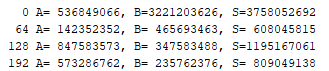
\includegraphics[width=.85\columnwidth]{ripple_adder_out}
                \caption*{Simulation - I : Normal Architecture}
            \end{center}
        \end{minipage}
        \begin{minipage}{.45\textwidth}
            \begin{center}
                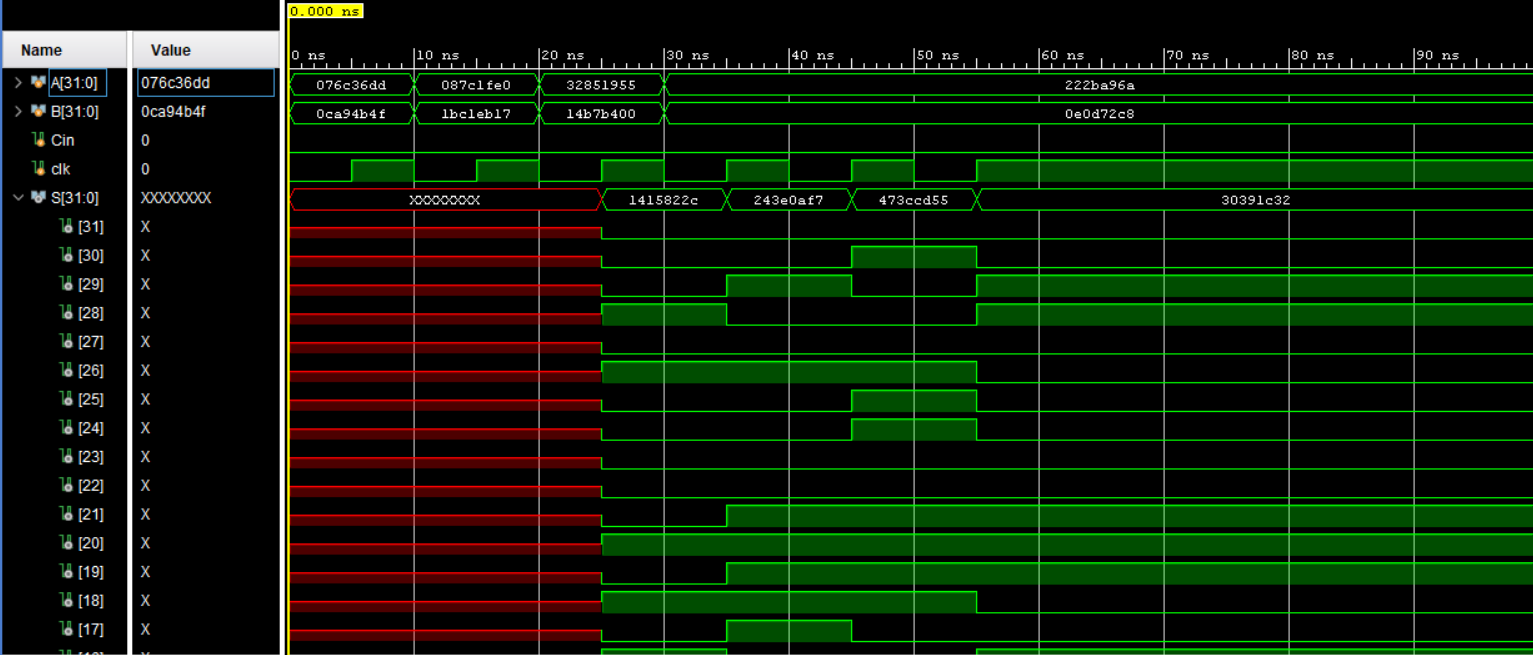
\includegraphics[width=.85\columnwidth]{pipeline_sim}
                \caption*{Simulation - II : Pipelined Architecture}
            \end{center}
        \end{minipage}
    \end{figure}

    \section{Carry Look-Ahead Adder}
    Instead of waiting for carry-bit to propagate through separate full adders, CLA implementation
    generates carry-bit parallelly with the price of a larger fan-in.
\vspace{-.25cm}
    \begin{align*}
        \text{Carry-Generate }\quad P_i &= A_i \oplus B_i\\
        \text{Carry-Propagate}\quad G_i &= A_i \cdot B_i\\
        \text{Carry-Bit} \quad  C_n &= C_0 \prod_{i=1}^{n-1}P_i+\sum_{i=0}^{n-1}\left\{ G_i \prod_{j=i+1}^{n-1}P_j \right\}
    \end{align*}
    In the case of an 8-bit adder, all the carry bits can be generated in an average time of 3$\tau$.
    Together with a delay of 2$\tau$ in the full adder, an 8-bit adder block takes 5$\tau$ to complete
    its process.
    Each block takes 2$\tau$ time to generate the carry-bit necessary for the next block and additionally
    the first stage takes $\tau$ time more to generate carry generate and propagate terms. Times add up
    to give a total delay of 11$\tau$ in the completion of addition between two 32-bit numbers.
    \begin{figure}[h]
        \begin{center}
            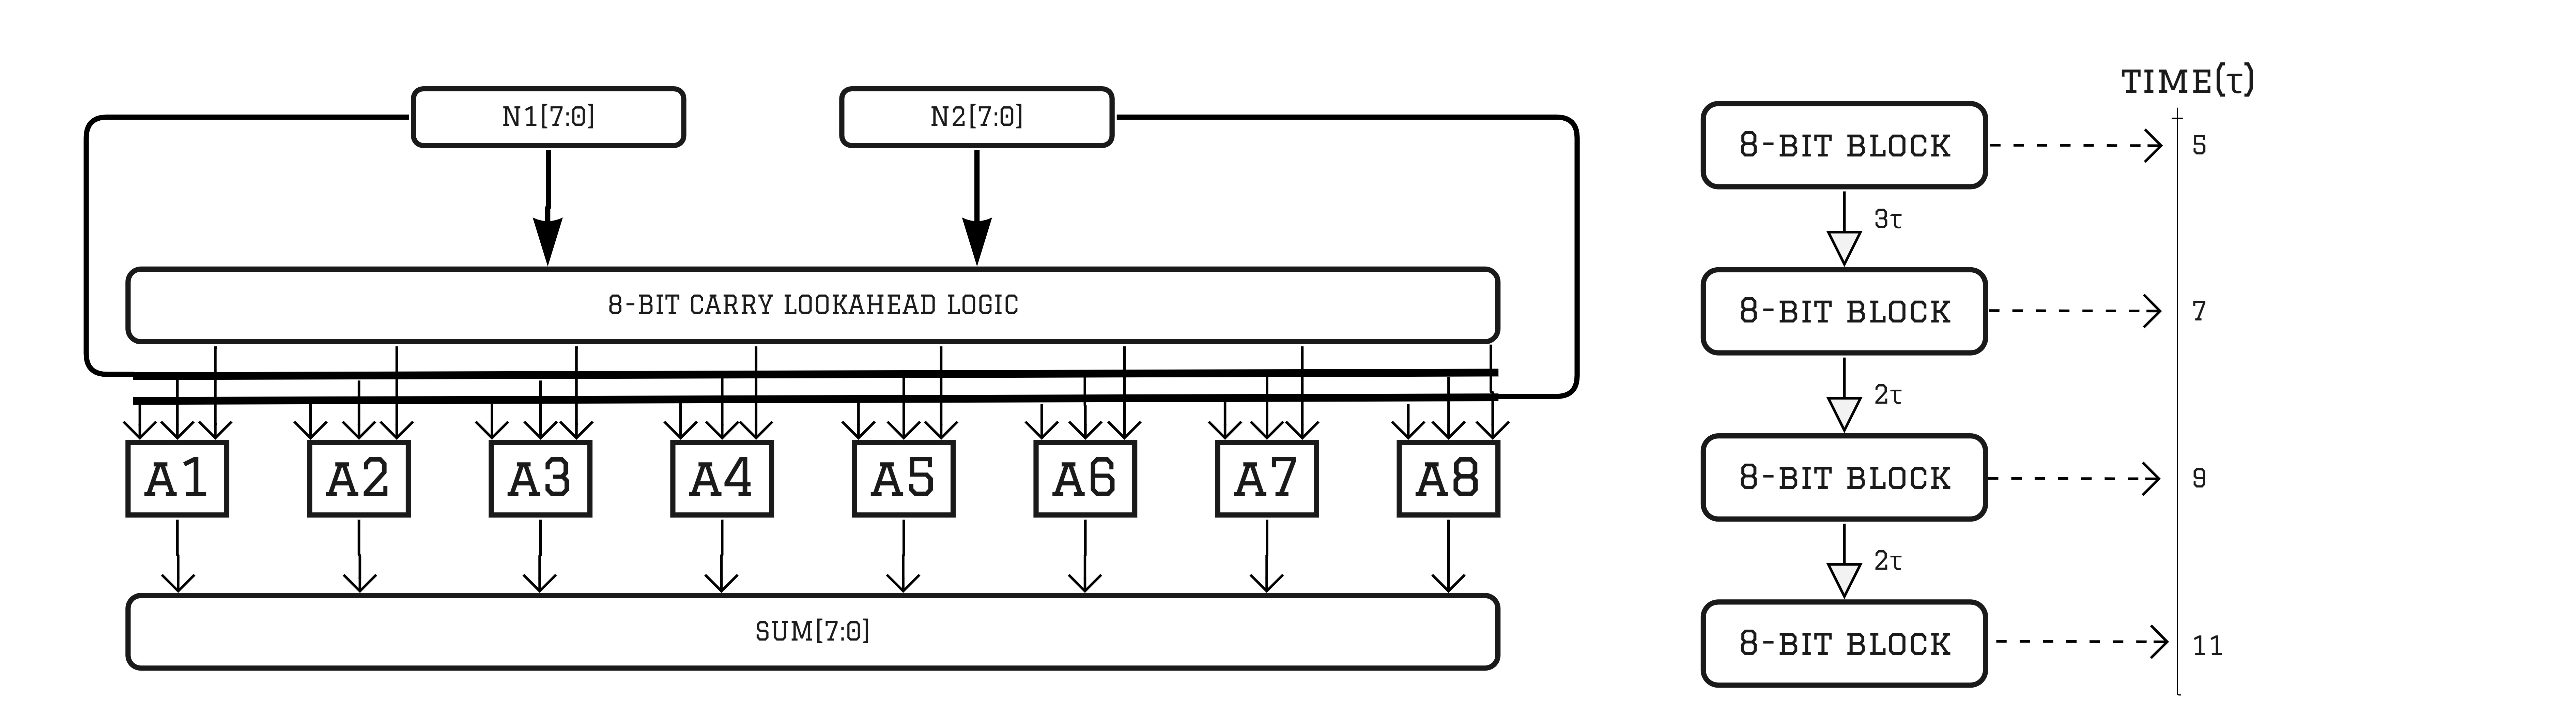
\includegraphics[width=.95\textwidth]{cla_adder}
            \caption*{Total time taken for the addition of four numbers = $4\times 11\tau = 44\tau$}
            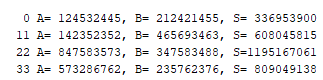
\includegraphics[width = .5\textwidth]{cla_adder_sim}
            \caption*{Simulation - III : CLA Architecture}
        \end{center}
    \end{figure}


    \section{Floating Point Addition/Subtraction}

    \subsection{IEEE-754 Single Precision Format}
    \begin{figure}[h]
        \begin{center}
            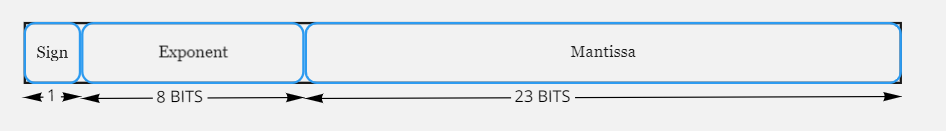
\includegraphics[width=.7\textwidth]{ieee}
        \end{center}
    \end{figure}
    For the verification purposes \href{https://www.h-schmidt.net/FloatConverter/IEEE754.html}{h-schmidt}, an online floatconverter is used.

    \subsection{Algorithm}
    \begin{enumerate}
        \item Compare the exponents of two numbers and find the absolute difference.
        \item Shift the number with the smaller exponent to right by the amount of absolute difference to make the exponents of both numbers equal. Assign the prominent exponent as the exponent of the sum.
        \item Check the signs of two numbers after performing sign conversion according to operation
        \begin{itemize}
            \item If both are of the same sign add two corresponding mantissa and assign it to sum\_mantissa.
            \item Otherwise, subtract the matissa of number with 1 as sign bit from the other and assign the magnitude of it as sum\_mantissa.
        \end{itemize}
        \hspace*{\dimexpr\linewidth-\textwidth\relax} At this stage, sum mantissa will contain 25 bits to accomadate the overflow.
        \item Assign the sum\_sign according to sign of two numbers and above derived answer.
        \item Shift the mantissa left until and 24th-bit position of the mantissa is one and reduce the exponent of the sum accordingly(normalization)
        \item Now discard the implicit 1 and consider only the lower 23-bits of sum\_mantissa.
        \item Final Answer = \{sum\_sign, sum\_exponent, sum\_mantissa\}
    \end{enumerate}
    \begin{figure}[h]
        \begin{center}
            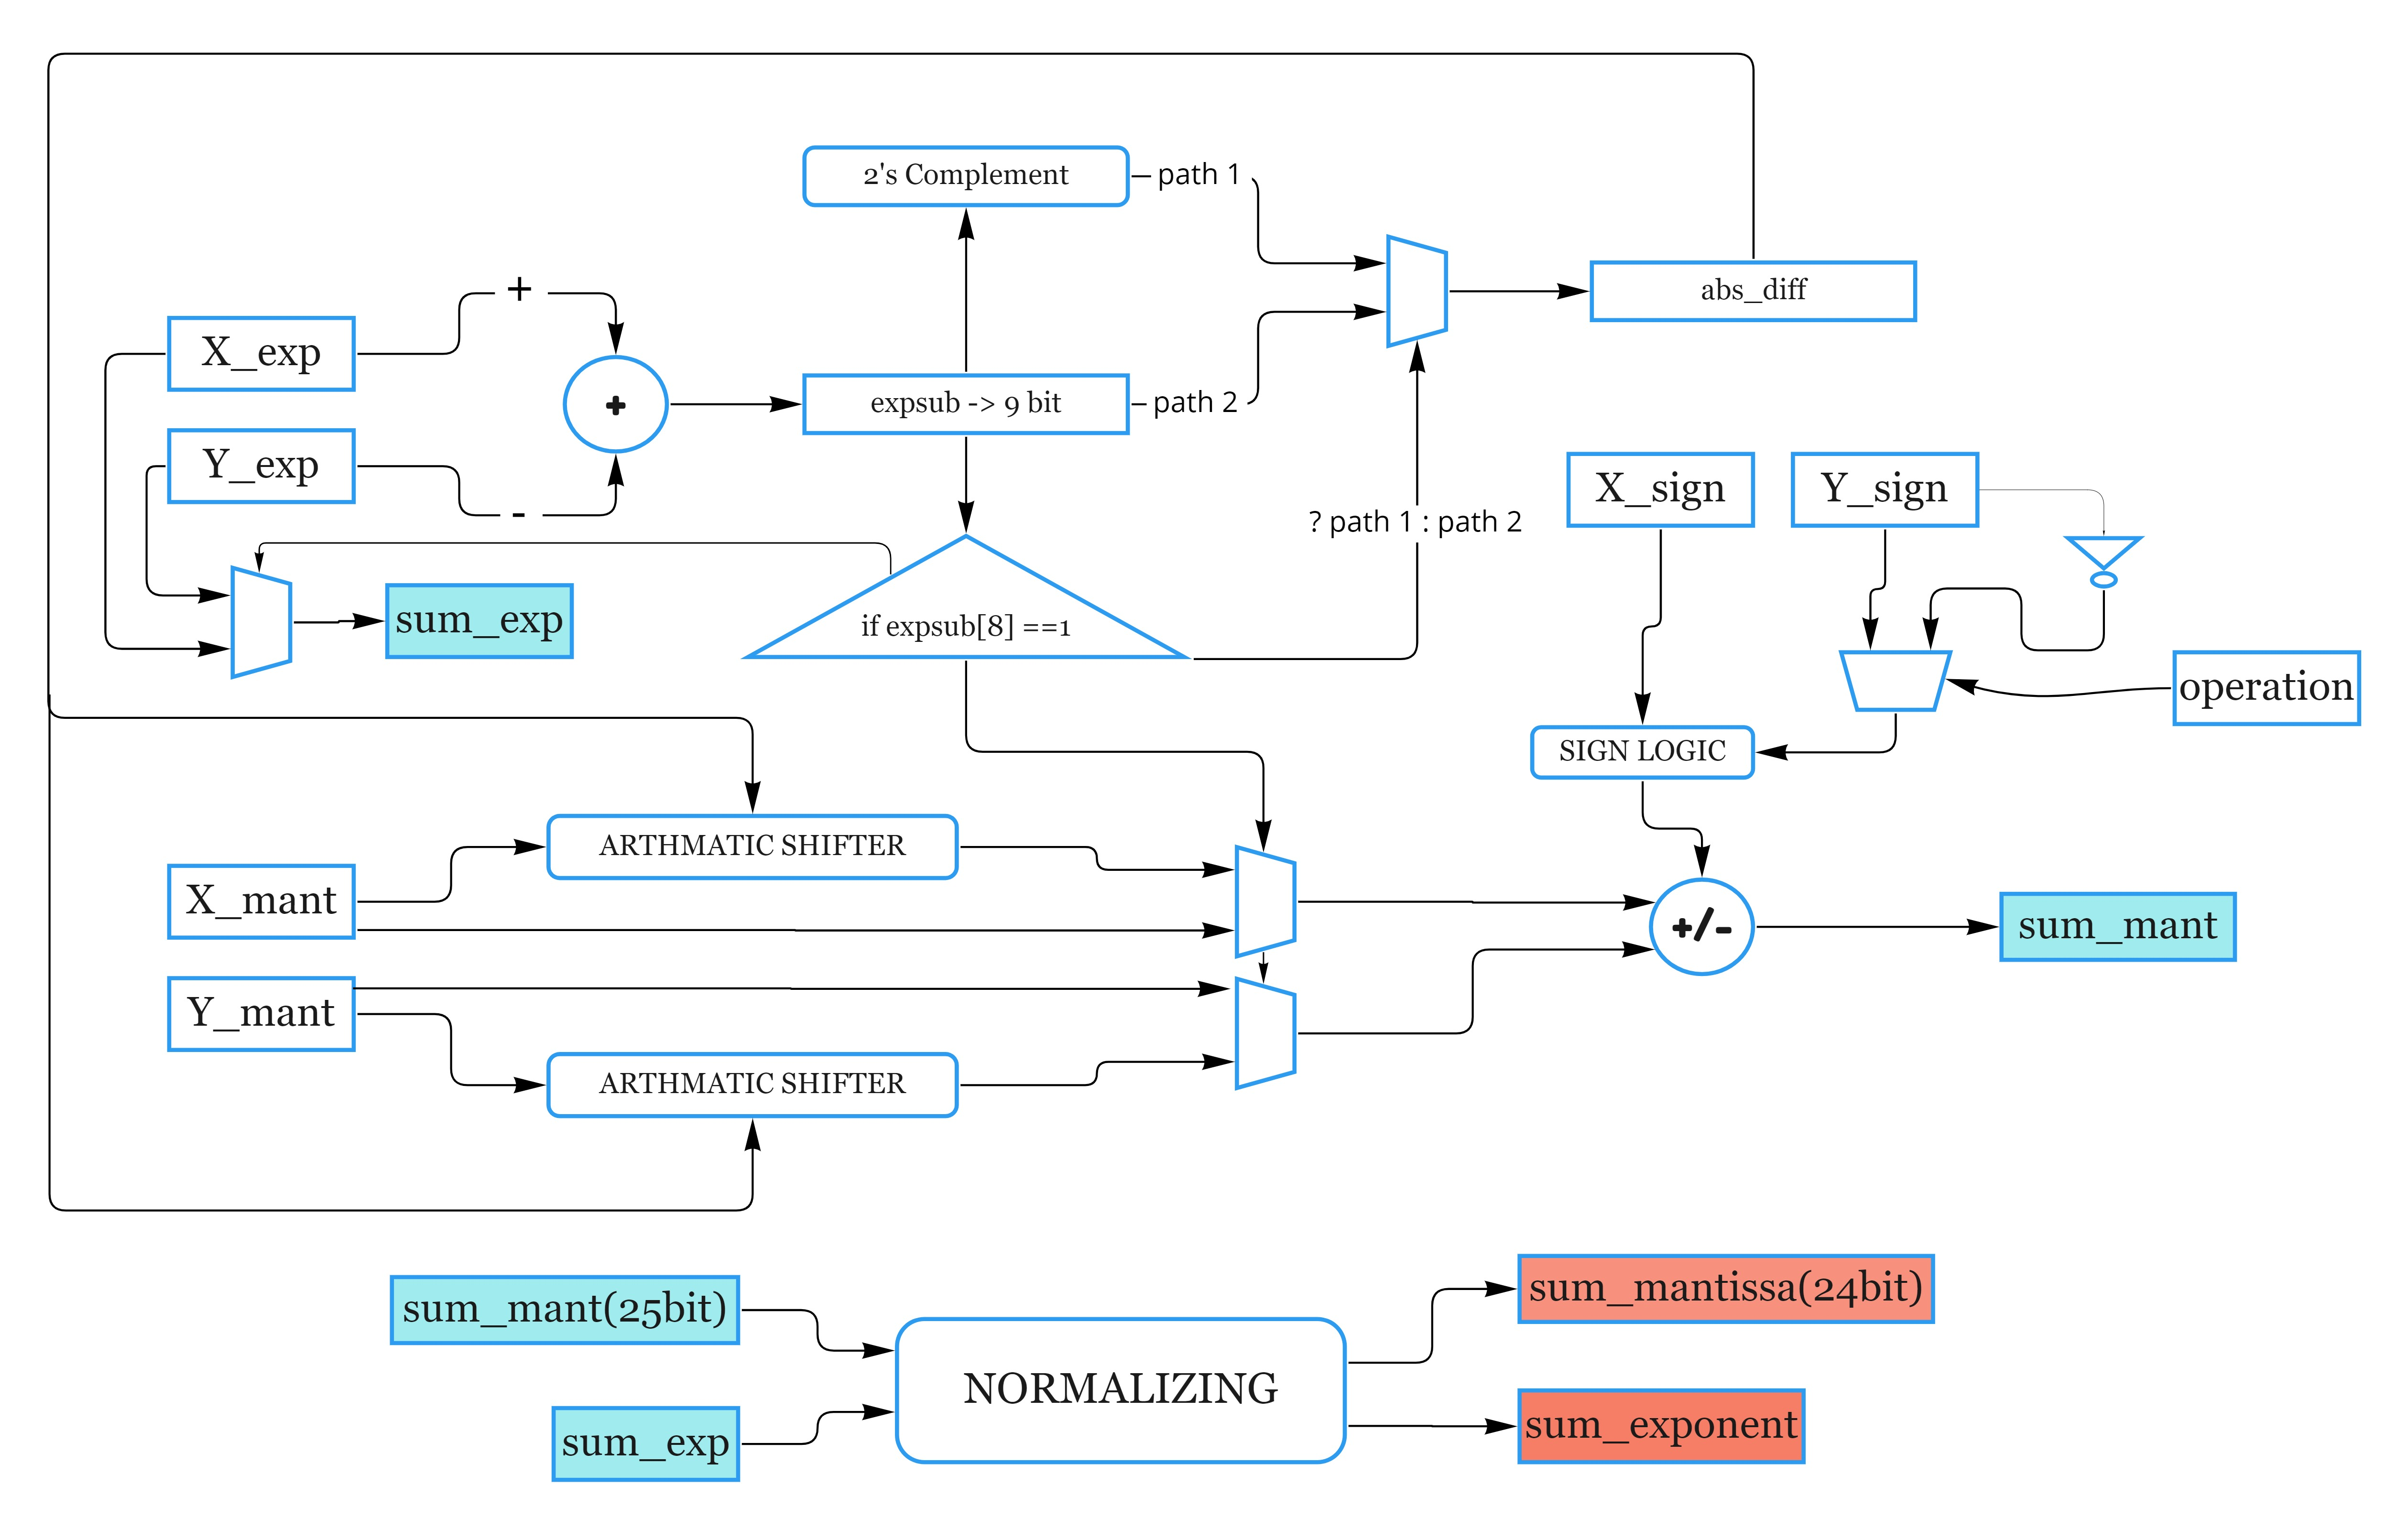
\includegraphics[width=.65\textwidth]{algorithm}
            \caption*{Design Flow of FP Add/Sub}
        \end{center}
    \end{figure}

    \subsection{Results}

    \begin{figure}[h]
        \caption*{Simulation Results}
        \begin{minipage}{.45\textwidth}
            \begin{center}
                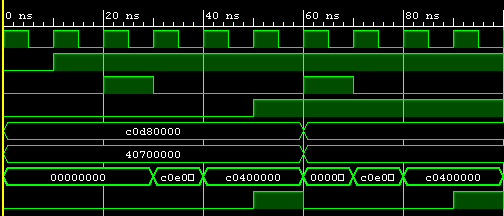
\includegraphics[width=.95\columnwidth]{operation-6.75_3.75}
                \caption*{-6.75+3.75 = -3 \& -6.75-(-3.75) = -3}
            \end{center}
        \end{minipage}
        \begin{minipage}{.45\textwidth}
            \begin{center}
                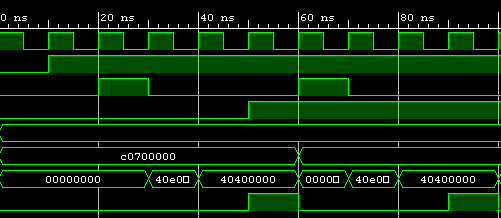
\includegraphics[width=.95\columnwidth]{6.75-3.75}
                \caption*{6.75-3.75 = 3 \& 6.75+(-3.75) = 3}
            \end{center}
        \end{minipage}

        \begin{minipage}{.45\textwidth}
            \begin{center}
                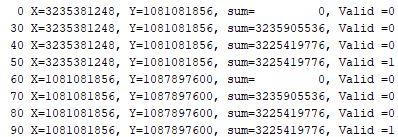
\includegraphics[width=.75\columnwidth]{ope_1}
            \end{center}
        \end{minipage}
        \begin{minipage}{.45\textwidth}
            \begin{center}
                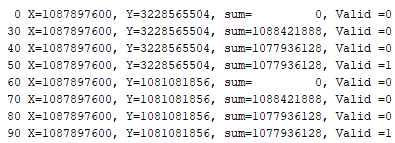
\includegraphics[width=.75\columnwidth]{ope_2}
            \end{center}
        \end{minipage}
    \end{figure}
    \vspace{.2cm}
    \newline
    Addition and Subtraction indicated above are choosen in a way to return the same result. During the true value of valid entry simulation returns same result for each operation.
    \newpage


    \section{Traffic Light Controller System : Borella Junction}
    The situation can be realized as four main states as shown in the figure below.
    \begin{figure}[h]
        \begin{minipage}{.24\textwidth}
            \begin{center}
                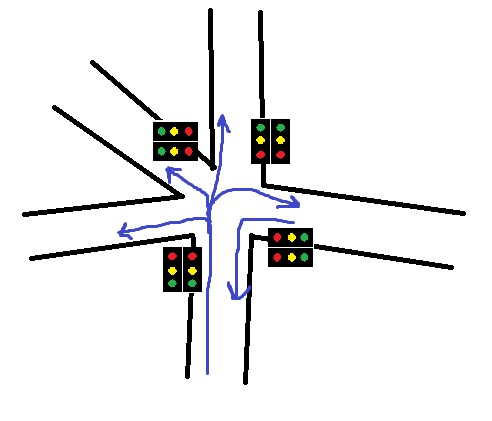
\includegraphics[width=\columnwidth]{state_1}
                \caption*{state : 1}
            \end{center}
        \end{minipage}
        \begin{minipage}{.24\textwidth}
            \begin{center}
                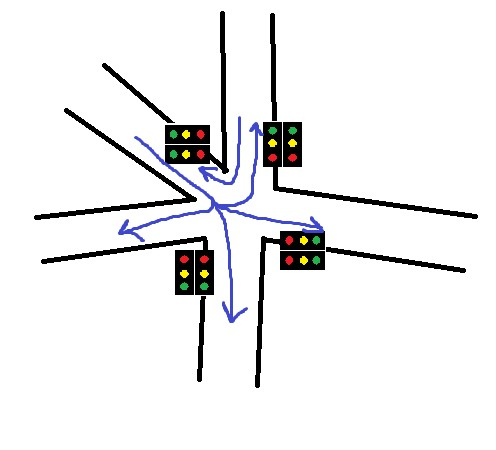
\includegraphics[width=\columnwidth]{state_2}
                \caption*{state : 2}
            \end{center}
        \end{minipage}
        \begin{minipage}{.24\textwidth}
            \begin{center}
                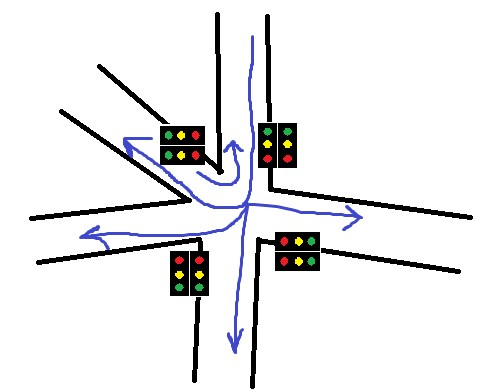
\includegraphics[width=\columnwidth]{state_3}
                \caption*{state : 3}
            \end{center}
        \end{minipage}
        \begin{minipage}{.24\textwidth}
            \begin{center}
                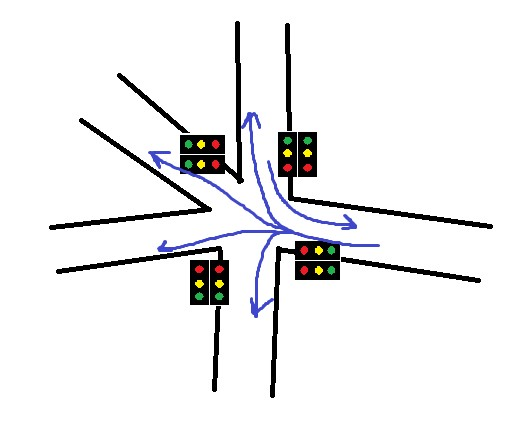
\includegraphics[width=\columnwidth]{state_4}
                \caption*{state : 4}
            \end{center}
        \end{minipage}
    \end{figure}
    \newline
    Transition between states properly done with no intersecting pathways having green at the same time.
    With these there are 12 states in total. These states can be realized using four flip-flops and required
    combinational circuitories. State Diagram illustrating all the 12 states is as follows.
    \begin{figure}[h]
               \centering
               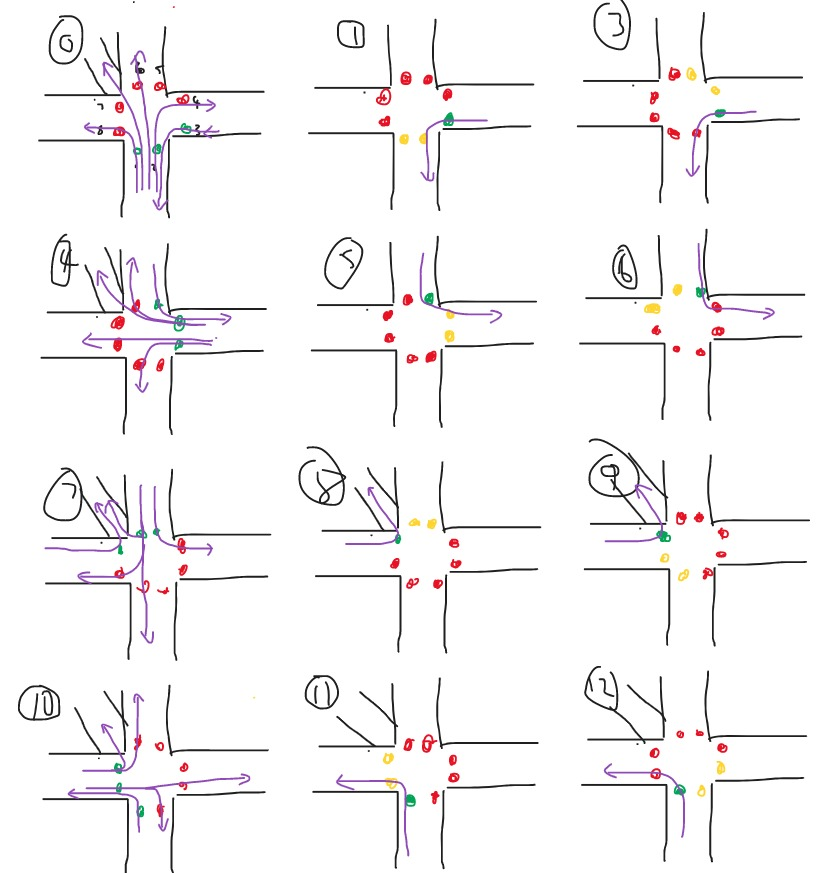
\includegraphics[width=.8\textwidth]{trafic_light}
        \caption*{State Diagram}
    \end{figure}

    \newline
    Pedestrain crossing is not considered as the Borella Junction has an underground crossing.
    A 10 bit counter is used, and throughout each full count the trasition between states happen sequentiall,
    and then the procedure will iterate.
    \newpage
    \begin{figure}[h]
        \centering
        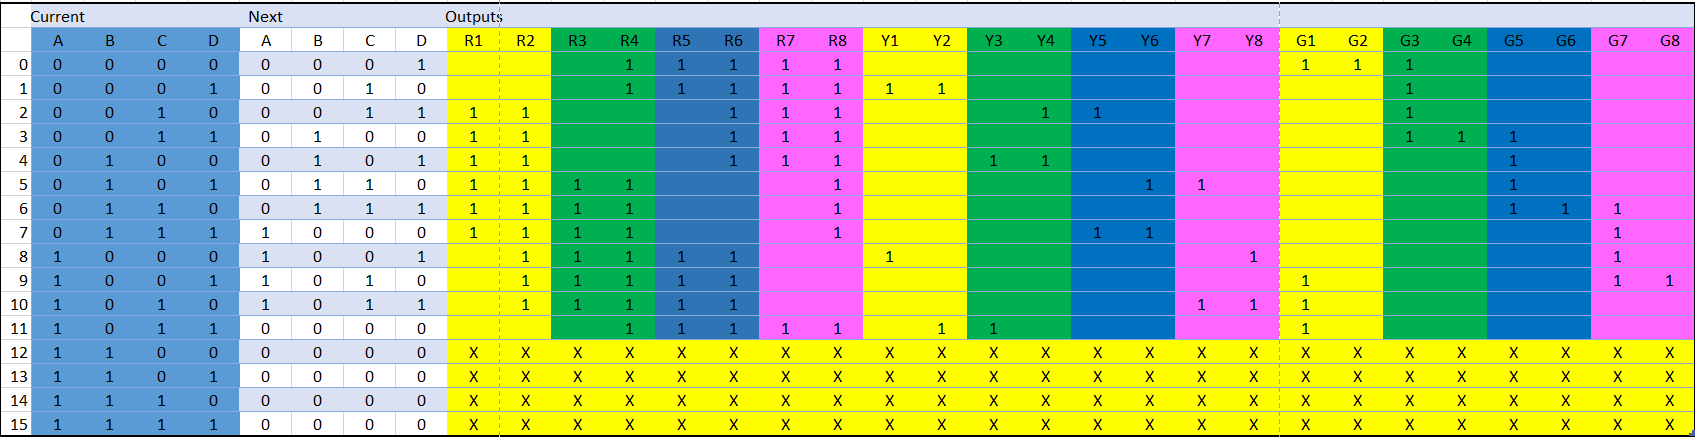
\includegraphics[width=\textwidth]{state_diagram}
        \caption*{Excitation Table of Different States}
    \end{figure}
Due to the larger size of variables, simulation results are not included with the report.
    
    \vfill
    
    \section*{References}
    \begin{enumerate}
        \item \href{https://esrd2014.blogspot.com/p/4-bit-carry-ripple-adder.html}{4-bit Carry Ripple Adder}
        \item \href{https://www.geeksforgeeks.org/carry-look-ahead-adder/}{Carry Look-Ahead Adder}
        \item \href{https://www.ijeat.org/wp-content/uploads/papers/v3i2/B2415123213.pdf}{Design and Comparative Analysis of Conventional
        Adder and Pipelined Adder}
        \item \href{https://github.com/ahirsharan/32-Bit-Floating-Point-Adder}{32-Bit-Floating-Point-Adder}
        \item \href{https://www.ijert.org/research/simulation-and-synthesis-model-for-the-addition-of-single-precision-floating-point-numbers-using-verilog-IJERTV2IS90913.pdf}{Simulation and Synthesis Model for the Addition of Single Precision
        Floating Point Numbers}
        \item \href{https://www.electrically4u.com/what-is-the-excitation-table/}{Excitation Table and State Diagram}
    \end{enumerate}

\end{document}
